\documentclass[11pt,letterpaper]{article}
\usepackage[T1]{fontenc}
\usepackage[scaled]{helvet}
\renewcommand{\familydefault}{\sfdefault}
\usepackage{amsmath,amssymb}
\usepackage[margin=0.8in,bottom=0.9in]{geometry}
\usepackage[most]{tcolorbox}
\usepackage{tikz}
\usetikzlibrary{calc}
\usepackage{enumitem}
\usepackage{array}
\usepackage{needspace}
\usepackage{fancyhdr}
\usepackage{pifont}

% ---- Palette "F. Bright & Playful" ----
\definecolor{fmtitle}{HTML}{3D2C8D}
\definecolor{fmkey}{HTML}{0096C7}
\definecolor{fmwatch}{HTML}{2BB673}
\definecolor{fmturn}{HTML}{F4A100}
\definecolor{fmmistake}{HTML}{EF476F}
\definecolor{fmnotice}{HTML}{9B5DE5}
\definecolor{fmgray}{HTML}{6B6B6B}

\pagestyle{fancy}
\fancyhf{}
\renewcommand{\headrulewidth}{0pt}
\fancyfoot[C]{\footnotesize\color{fmgray}\textcopyright\ 2026 FangMath. All rights reserved.}
\fancyfoot[R]{\footnotesize\color{fmgray}\thepage}
\setlength{\parindent}{0pt}
\setlength{\parskip}{3pt}

\newcommand{\badge}[1]{\colorbox{fmtitle}{\color{white}\bfseries\small\ #1\ }}
\newcommand{\leveltag}[2]{\colorbox{#1}{\color{white}\bfseries\scriptsize\ #2\ }}
\newcommand{\LE}{\leveltag{fmwatch}{EASY}}
\newcommand{\LM}{\leveltag{fmturn}{MEDIUM}}
\newcommand{\LH}{\leveltag{fmmistake}{HARD}}

\newcommand{\sectionbar}[2]{\needspace{6cm}\par\vspace{4mm}
  \begin{tcolorbox}[enhanced,colback=fmtitle,colframe=fmtitle,arc=2mm,
    left=4mm,top=1.5mm,bottom=1.5mm]
  \color{white}\bfseries\large #1\hfill{\normalsize\mdseries #2}
  \end{tcolorbox}}

\newtcolorbox{keyidea}{enhanced,breakable,colback=white,colframe=fmkey,boxrule=1pt,arc=2mm,
  title={Key Idea},coltitle=fmkey,fonttitle=\bfseries,
  attach boxed title to top left={xshift=4mm,yshift=-2mm},
  boxed title style={colback=white,colframe=fmkey,boxrule=0.9pt}}
\newtcolorbox{watchme}{enhanced,colback=white,colframe=fmwatch,boxrule=1pt,arc=2mm,
  title={Watch Me --- Worked Example},coltitle=fmwatch,fonttitle=\bfseries,
  attach boxed title to top left={xshift=4mm,yshift=-2mm},
  boxed title style={colback=white,colframe=fmwatch,boxrule=0.9pt}}
\newtcolorbox{mistakebox}{enhanced,breakable,colback=white,colframe=fmmistake,boxrule=1pt,arc=2mm,
  title={Common Mistake},coltitle=fmmistake,fonttitle=\bfseries,
  attach boxed title to top left={xshift=4mm,yshift=-2mm},
  boxed title style={colback=white,colframe=fmmistake,boxrule=0.9pt}}
\newtcolorbox{yourturn}{enhanced,breakable,colback=white,colframe=fmturn,boxrule=1pt,arc=2mm,
  title={Your Turn},coltitle=fmturn,fonttitle=\bfseries,
  attach boxed title to top left={xshift=4mm,yshift=-2mm},
  boxed title style={colback=white,colframe=fmturn,boxrule=0.9pt}}
\newtcolorbox{answerbox}[1]{enhanced,breakable,colback=white,colframe=fmwatch,boxrule=1pt,arc=2mm,
  title={#1},coltitle=fmwatch,fonttitle=\bfseries,
  attach boxed title to top left={xshift=4mm,yshift=-2mm},
  boxed title style={colback=white,colframe=fmwatch,boxrule=0.9pt}}

\newcommand{\work}[1]{\par\vspace{#1}}
\setlist[enumerate]{itemsep=2pt,topsep=3pt}

% ---------------- extra boxes ----------------
\newtcolorbox{notebox}{enhanced,breakable,colback=white,colframe=fmnotice,boxrule=1pt,arc=2mm,
  title={Notice},coltitle=fmnotice,fonttitle=\bfseries,
  attach boxed title to top left={xshift=4mm,yshift=-2mm},
  boxed title style={colback=white,colframe=fmnotice,boxrule=0.9pt}}
\newtcolorbox{exbox}{enhanced,colback=white,colframe=fmwatch,boxrule=0.8pt,arc=2mm,
  title={Example},coltitle=fmwatch,fonttitle=\bfseries\small,
  attach boxed title to top left={xshift=4mm,yshift=-2mm},
  boxed title style={colback=white,colframe=fmwatch,boxrule=0.8pt},fontupper=\small}
\newcommand{\topicbar}[1]{\needspace{4.5cm}\par\vspace{5mm}
  \begin{tcolorbox}[enhanced,colback=fmtitle,colframe=fmtitle,arc=2mm,left=4mm,top=1.5mm,bottom=1.5mm]
  \color{white}\bfseries\large #1
  \end{tcolorbox}}
\usepackage{multicol}

% ---------------- practice layout ----------------
\newcommand{\workline}{\par\vspace{7mm}{\color{gray!55}\rule{\linewidth}{0.4pt}}}
\newcommand{\worklines}[1]{\foreach \i in {1,...,#1}{\workline}}
\newcommand{\prob}[3]{\needspace{#3}\par\vspace{3mm}{\color{fmturn}\bfseries #1.}\ #2\par}
\newcommand{\ansline}{\par\vspace{4mm}\hfill\textbf{Answer:}\ \rule{5cm}{0.4pt}\par}
\newcommand{\keyitem}[3]{\needspace{3.2cm}\par\vspace{2mm}
  \begin{tcolorbox}[enhanced,colback=white,colframe=fmwatch!60,boxrule=0.6pt,arc=1.5mm,left=3mm,top=1.5mm,bottom=1.5mm]
  {\color{fmwatch}\bfseries #1.}\quad\small #2\par\vspace{1mm}
  \normalsize\textbf{Answer: #3}
  \end{tcolorbox}}



\newcommand{\grid}[1][0.32]{\begin{tikzpicture}[scale=#1]
 \draw[gray!30,thin] (-6,-6) grid (6,6);
 \draw[->,thick] (-6.4,0)--(6.5,0) node[right,font=\scriptsize]{$x$};
 \draw[->,thick] (0,-6.4)--(0,6.5) node[above,font=\scriptsize]{$y$};
 
\end{tikzpicture}}

\begin{document}
\badge{WORKSHEET}\hfill{\small\color{fmgray}Algebra 1 \textperiodcentered\ Systems of Equations}\par\vspace{4mm}
{\color{fmtitle}\LARGE\bfseries Systems of Linear Equations}\par\vspace{1mm}
{\color{fmgray}30 problems \textperiodcentered\ A worked example comes before each type. Show every step.}\par\vspace{3mm}
Name: \rule{6cm}{0.4pt}\hspace{1cm}Date: \rule{3.5cm}{0.4pt}\par\vspace{1mm}

\begin{keyidea}A \textbf{system} is two equations at the same time. Its \textbf{solution} is the point $(x, y)$ that makes \textbf{both} equations true --- where the two lines cross.
\begin{itemize}[itemsep=1pt,topsep=2pt]
\item \textbf{Graphing}: draw both lines and read the crossing point.
\item \textbf{Substitution}: one equation already says ``$y = \ldots$'' (or $x = \ldots$)? Put it into the other.
\item \textbf{Elimination}: add or subtract the equations so one letter disappears.
\end{itemize}\end{keyidea}
\begin{mistakebox}A solution must work in \textbf{both} equations --- always check in the one you did \emph{not} use last.\par
When you subtract an equation, subtract \emph{every} term: $(3x + 2y) - (x - 2y) = 2x + 4y$, \textbf{not} $2x$.\end{mistakebox}
\needspace{9cm}\topicbar{Type 1 \quad Is It a Solution?}
\begin{watchme}\textbf{Is $(4, 1)$ a solution of \ $x + y = 5$ \ and \ $x - y = 3$?}\par\vspace{1mm}Put $x = 4$, $y = 1$ into \textbf{both} equations.\par\vspace{1mm}
\renewcommand{\arraystretch}{2.0}\begin{tabular}{@{}l l@{}}
\textbf{Equation 1} & $4 + 1 = 5$ \ \ding{51}\\
\textbf{Equation 2} & $4 - 1 = 3$ \ \ding{51}\\
\textbf{Answer} & \textbf{Yes} --- it works in both.
\end{tabular}\end{watchme}
\needspace{3.3cm}\par\vspace{3mm}\noindent \begin{minipage}[t][2.8cm]{0.48\linewidth}\raggedright{\color{fmturn}\bfseries 1.}\ Is $(2, 3)$ a solution of \\ $x + y = 5$ \ and \ $2x - y = 1$?\par\vfill\hfill Yes / No:\ \rule{3.2cm}{0.4pt}\end{minipage}\hfill \begin{minipage}[t][2.8cm]{0.48\linewidth}\raggedright{\color{fmturn}\bfseries 2.}\ Is $(1, 4)$ a solution of \\ $y = 3x + 1$ \ and \ $x + y = 6$?\par\vfill\hfill Yes / No:\ \rule{3.2cm}{0.4pt}\end{minipage}\par
\needspace{3.3cm}\par\vspace{3mm}\noindent \begin{minipage}[t][2.8cm]{0.48\linewidth}\raggedright{\color{fmturn}\bfseries 3.}\ Is $(-1, 2)$ a solution of \\ $2x + 3y = 4$ \ and \ $y = -2x$?\par\vfill\hfill Yes / No:\ \rule{3.2cm}{0.4pt}\end{minipage}\hfill \begin{minipage}[t][2.8cm]{0.48\linewidth}\raggedright{\color{fmturn}\bfseries 4.}\ Is $(3, -2)$ a solution of \\ $x - y = 5$ \ and \ $x + 2y = 1$?\par\vfill\hfill Yes / No:\ \rule{3.2cm}{0.4pt}\end{minipage}\par
\needspace{9cm}\topicbar{Type 2 \quad Solve by Graphing}
\begin{watchme}\textbf{Solve by graphing: \ $y = x + 1$ \ and \ $y = -x + 3$.}\par\vspace{1mm}\begin{minipage}[c]{0.55\linewidth}\renewcommand{\arraystretch}{2.0}\begin{tabular}{@{}l l@{}}\textbf{Step 1} & Graph $y = x + 1$: start at $(0, 1)$, up 1, right 1.\\ \textbf{Step 2} & Graph $y = -x + 3$: start at $(0, 3)$, down 1, right 1.\\\textbf{Step 3} & They cross at $(1, 2)$. Check: $2 = 1 + 1$, \ $2 = -1 + 3$.\\ \textbf{Answer} & $\boldsymbol{(1, 2)}$\end{tabular}\end{minipage}\hfill\begin{minipage}[c]{0.4\linewidth}\centering 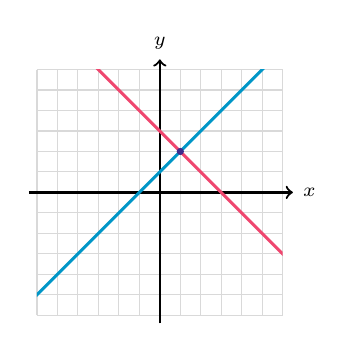
\begin{tikzpicture}[scale=0.26]
\draw[gray!30,thin] (-6,-6) grid (6,6);
\draw[->,thick] (-6.4,0)--(6.5,0) node[right,font=\scriptsize]{$x$};
\draw[->,thick] (0,-6.4)--(0,6.5) node[above,font=\scriptsize]{$y$};
\begin{scope}\clip (-6,-6) rectangle (6,6);
\draw[fmkey,line width=1.1pt] (-7,-6.000)--(7,8.000);
\draw[fmmistake,line width=1.1pt] (-7,10.000)--(7,-4.000);
\end{scope}
\fill[fmtitle] (1.0,2.0) circle (5pt);
\end{tikzpicture}\end{minipage}\end{watchme}
\needspace{6.2cm}\par\vspace{3mm}\noindent \begin{minipage}[t]{0.48\linewidth}\raggedright{\color{fmturn}\bfseries 5.}\ Solve by graphing: \ $y = x + 1$ \ and \ $y = -x + 5$.\par\vspace{1mm}\centering 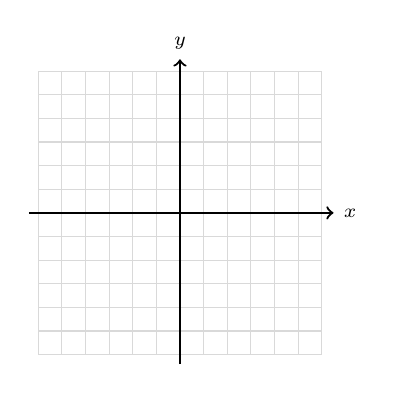
\begin{tikzpicture}[scale=0.3]
\draw[gray!30,thin] (-6,-6) grid (6,6);
\draw[->,thick] (-6.4,0)--(6.5,0) node[right,font=\scriptsize]{$x$};
\draw[->,thick] (0,-6.4)--(0,6.5) node[above,font=\scriptsize]{$y$};
\begin{scope}\clip (-6,-6) rectangle (6,6);
\end{scope}
\end{tikzpicture}\end{minipage}\hfill \begin{minipage}[t]{0.48\linewidth}\raggedright{\color{fmturn}\bfseries 6.}\ Solve by graphing: \ $y = \dfrac{1}{2}x - 2$ \ and \ $y = -x + 4$.\par\vspace{1mm}\centering 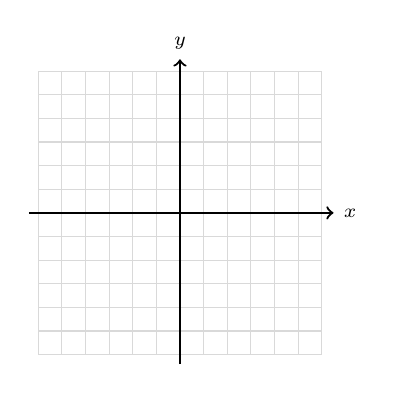
\begin{tikzpicture}[scale=0.3]
\draw[gray!30,thin] (-6,-6) grid (6,6);
\draw[->,thick] (-6.4,0)--(6.5,0) node[right,font=\scriptsize]{$x$};
\draw[->,thick] (0,-6.4)--(0,6.5) node[above,font=\scriptsize]{$y$};
\begin{scope}\clip (-6,-6) rectangle (6,6);
\end{scope}
\end{tikzpicture}\end{minipage}\par
\needspace{6.2cm}\par\vspace{3mm}\noindent \begin{minipage}[t]{0.48\linewidth}\raggedright{\color{fmturn}\bfseries 7.}\ Solve by graphing: \ $y = 2x - 3$ \ and \ $y = -x + 3$.\par\vspace{1mm}\centering 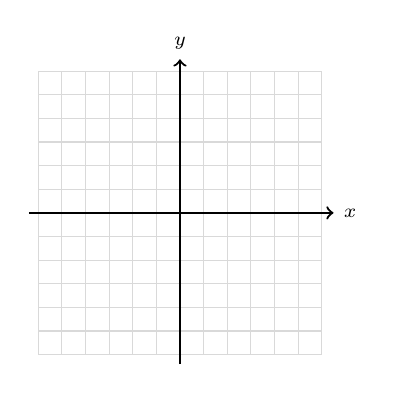
\begin{tikzpicture}[scale=0.3]
\draw[gray!30,thin] (-6,-6) grid (6,6);
\draw[->,thick] (-6.4,0)--(6.5,0) node[right,font=\scriptsize]{$x$};
\draw[->,thick] (0,-6.4)--(0,6.5) node[above,font=\scriptsize]{$y$};
\begin{scope}\clip (-6,-6) rectangle (6,6);
\end{scope}
\end{tikzpicture}\end{minipage}\hfill \begin{minipage}[t]{0.48\linewidth}\raggedright{\color{fmturn}\bfseries 8.}\ Solve by graphing: \ $y = -x + 1$ \ and \ $y = x - 3$.\par\vspace{1mm}\centering 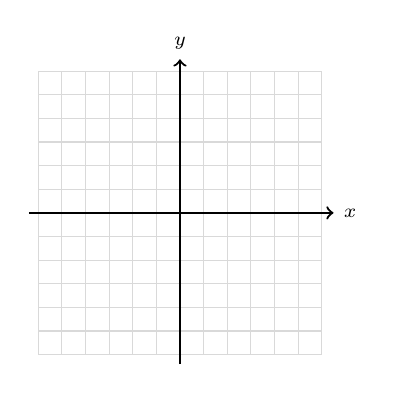
\begin{tikzpicture}[scale=0.3]
\draw[gray!30,thin] (-6,-6) grid (6,6);
\draw[->,thick] (-6.4,0)--(6.5,0) node[right,font=\scriptsize]{$x$};
\draw[->,thick] (0,-6.4)--(0,6.5) node[above,font=\scriptsize]{$y$};
\begin{scope}\clip (-6,-6) rectangle (6,6);
\end{scope}
\end{tikzpicture}\end{minipage}\par
\needspace{9cm}\topicbar{Type 3 \quad Substitution}
\begin{watchme}\textbf{Solve: \ $y = 3x$ \ and \ $x + y = 8$.}\par\vspace{1mm}The first equation tells you what $y$ is. Replace $y$ in the second equation with $3x$.\par\vspace{1mm}
\renewcommand{\arraystretch}{2.0}\begin{tabular}{@{}l l@{}}
\textbf{Step 1 \ Substitute} & $x + 3x = 8$\\
\textbf{Step 2 \ Solve} & $4x = 8$, \ $x = 2$\\
\textbf{Step 3 \ Find $y$} & $y = 3 \cdot 2 = 6$\\
\textbf{Check} & $2 + 6 = 8$ \ \ding{51}\\
\textbf{Answer} & $\boldsymbol{(2, 6)}$
\end{tabular}\end{watchme}
\needspace{3.9cm}\par\vspace{3mm}\noindent \begin{minipage}[t][3.4cm]{0.48\linewidth}\raggedright{\color{fmturn}\bfseries 9.}\ Solve: \ $y = 2x$ \ and \ $x + y = 12$\par\vfill\hfill $(x, y) =$\ \rule{3.2cm}{0.4pt}\end{minipage}\hfill \begin{minipage}[t][3.4cm]{0.48\linewidth}\raggedright{\color{fmturn}\bfseries 10.}\ Solve: \ $y = x + 3$ \ and \ $2x + y = 9$\par\vfill\hfill $(x, y) =$\ \rule{3.2cm}{0.4pt}\end{minipage}\par
\needspace{3.9cm}\par\vspace{3mm}\noindent \begin{minipage}[t][3.4cm]{0.48\linewidth}\raggedright{\color{fmturn}\bfseries 11.}\ Solve: \ $x = y - 1$ \ and \ $3x + y = 13$\par\vfill\hfill $(x, y) =$\ \rule{3.2cm}{0.4pt}\end{minipage}\hfill \begin{minipage}[t][3.4cm]{0.48\linewidth}\raggedright{\color{fmturn}\bfseries 12.}\ Solve: \ $y = -3x + 2$ \ and \ $x - y = 6$\par\vfill\hfill $(x, y) =$\ \rule{3.2cm}{0.4pt}\end{minipage}\par
\needspace{3.9cm}\par\vspace{3mm}\noindent \begin{minipage}[t][3.4cm]{0.48\linewidth}\raggedright{\color{fmturn}\bfseries 13.}\ Solve: \ $y = 4x - 5$ \ and \ $y = 2x + 1$\par\vfill\hfill $(x, y) =$\ \rule{3.2cm}{0.4pt}\end{minipage}\hfill \begin{minipage}[t][3.4cm]{0.48\linewidth}\raggedright{\color{fmturn}\bfseries 14.}\ Solve: \ $x + 2y = 7$ \ and \ $x = 3y - 8$\par\vfill\hfill $(x, y) =$\ \rule{3.2cm}{0.4pt}\end{minipage}\par
\needspace{9cm}\topicbar{Type 4 \quad Elimination}
\begin{watchme}\textbf{Solve: \ $3x + 2y = 16$ \ and \ $x - 2y = 0$.}\par\vspace{1mm}The $y$-terms are $+2y$ and $-2y$: adding the equations makes $y$ disappear.\par\vspace{1mm}
\renewcommand{\arraystretch}{2.0}\begin{tabular}{@{}l l@{}}
\textbf{Step 1 \ Add the equations} & $4x = 16$\\
\textbf{Step 2 \ Solve} & $x = 4$\\
\textbf{Step 3 \ Find $y$} & $4 - 2y = 0$, \ $y = 2$\\
\textbf{Check} & $3 \cdot 4 + 2 \cdot 2 = 16$ \ \ding{51}\\
\textbf{Answer} & $\boldsymbol{(4, 2)}$
\end{tabular}\end{watchme}
\begin{notebox}No opposite terms? \textbf{Multiply first.} In $x + 2y = 8$ and $3x + 4y = 20$, multiply the first equation by 2 so both have $4y$, then subtract.\end{notebox}
\needspace{3.9cm}\par\vspace{3mm}\noindent \begin{minipage}[t][3.4cm]{0.48\linewidth}\raggedright{\color{fmturn}\bfseries 15.}\ Solve: \ $x + y = 10$ \ and \ $x - y = 4$\par\vfill\hfill $(x, y) =$\ \rule{3.2cm}{0.4pt}\end{minipage}\hfill \begin{minipage}[t][3.4cm]{0.48\linewidth}\raggedright{\color{fmturn}\bfseries 16.}\ Solve: \ $2x + 3y = 13$ \ and \ $2x - y = 1$\par\vfill\hfill $(x, y) =$\ \rule{3.2cm}{0.4pt}\end{minipage}\par
\needspace{3.9cm}\par\vspace{3mm}\noindent \begin{minipage}[t][3.4cm]{0.48\linewidth}\raggedright{\color{fmturn}\bfseries 17.}\ Solve: \ $3x + y = 11$ \ and \ $x - y = 1$\par\vfill\hfill $(x, y) =$\ \rule{3.2cm}{0.4pt}\end{minipage}\hfill \begin{minipage}[t][3.4cm]{0.48\linewidth}\raggedright{\color{fmturn}\bfseries 18.}\ Solve: \ $x + 2y = 8$ \ and \ $3x + 4y = 20$\par\vfill\hfill $(x, y) =$\ \rule{3.2cm}{0.4pt}\end{minipage}\par
\needspace{3.9cm}\par\vspace{3mm}\noindent \begin{minipage}[t][3.4cm]{0.48\linewidth}\raggedright{\color{fmturn}\bfseries 19.}\ Solve: \ $2x + y = 7$ \ and \ $3x - 2y = 7$\par\vfill\hfill $(x, y) =$\ \rule{3.2cm}{0.4pt}\end{minipage}\hfill \begin{minipage}[t][3.4cm]{0.48\linewidth}\raggedright{\color{fmturn}\bfseries 20.}\ Solve: \ $4x + 3y = 1$ \ and \ $2x - y = 3$\par\vfill\hfill $(x, y) =$\ \rule{3.2cm}{0.4pt}\end{minipage}\par
\needspace{9cm}\topicbar{Type 5 \quad How Many Solutions?}
\begin{watchme}\textbf{Compare slopes and $y$-intercepts --- no need to solve.}\par\vspace{1mm}\renewcommand{\arraystretch}{1.6}\begin{tabular}{@{}l l l@{}}\textbf{Slopes} & \textbf{$y$-intercepts} & \textbf{Solutions}\\ \hline different & --- & \textbf{one} (the lines cross)\\ same & different & \textbf{none} (parallel lines)\\ same & same & \textbf{infinitely many} (the same line)\end{tabular}\par\vspace{2mm}\textbf{Example:} $y = 2x + 3$ and $y = 2x - 1$: same slope 2, different intercepts $\Rightarrow$ \textbf{no solution}.\end{watchme}
\needspace{3.1cm}\par\vspace{3mm}\noindent \begin{minipage}[t][2.6cm]{0.48\linewidth}\raggedright{\color{fmturn}\bfseries 21.}\ How many solutions? \\ $y = 2x + 1$ \ and \ $y = 2x - 4$\par\vfill\hfill Answer:\ \rule{3.2cm}{0.4pt}\end{minipage}\hfill \begin{minipage}[t][2.6cm]{0.48\linewidth}\raggedright{\color{fmturn}\bfseries 22.}\ How many solutions? \\ $y = 3x - 2$ \ and \ $y = -x + 6$\par\vfill\hfill Answer:\ \rule{3.2cm}{0.4pt}\end{minipage}\par
\needspace{3.1cm}\par\vspace{3mm}\noindent \begin{minipage}[t][2.6cm]{0.48\linewidth}\raggedright{\color{fmturn}\bfseries 23.}\ How many solutions? \\ $y = \tfrac12 x + 3$ \ and \ $2y = x + 6$\par\vfill\hfill Answer:\ \rule{3.2cm}{0.4pt}\end{minipage}\hfill \begin{minipage}[t][2.6cm]{0.48\linewidth}\raggedright{\color{fmturn}\bfseries 24.}\ How many solutions? \\ $x + y = 5$ \ and \ $x + y = 9$\par\vfill\hfill Answer:\ \rule{3.2cm}{0.4pt}\end{minipage}\par
\needspace{3.1cm}\par\vspace{3mm}\noindent \begin{minipage}[t][2.6cm]{0.48\linewidth}\raggedright{\color{fmturn}\bfseries 25.}\ How many solutions? \\ $3x - y = 2$ \ and \ $6x - 2y = 4$\par\vfill\hfill Answer:\ \rule{3.2cm}{0.4pt}\end{minipage}\hfill \begin{minipage}[t][2.6cm]{0.48\linewidth}\raggedright{\color{fmturn}\bfseries 26.}\ How many solutions? \\ $y = -4x + 1$ \ and \ $y = 4x + 1$\par\vfill\hfill Answer:\ \rule{3.2cm}{0.4pt}\end{minipage}\par
\needspace{9cm}\topicbar{Type 6 \quad Word Problems}
\begin{watchme}\textbf{Adult tickets cost \$8 and child tickets cost \$5. A family buys 6 tickets for \$39. How many of each?}\par\vspace{1mm}Two unknowns, two facts: one equation for \textbf{how many}, one for \textbf{how much money}. Let $a$ = adults, $c$ = children.\par\vspace{1mm}
\renewcommand{\arraystretch}{2.0}\begin{tabular}{@{}l l@{}}
\textbf{Step 1 \ How many} & $a + c = 6$\\
\textbf{Step 2 \ How much} & $8a + 5c = 39$\\
\textbf{Step 3 \ Substitute $c = 6 - a$} & $8a + 30 - 5a = 39$, \ $3a = 9$, \ $a = 3$\\
\textbf{Answer} & \textbf{3 adult and 3 child tickets} \ (check: $24 + 15 = 39$)
\end{tabular}\end{watchme}
\needspace{3.9cm}\par\vspace{3mm}\noindent \begin{minipage}[t][3.4cm]{0.48\linewidth}\raggedright{\color{fmturn}\bfseries 27.}\ The sum of two numbers is 20 and their difference is 6. Find the numbers.\par\vfill\hfill Answer:\ \rule{3.2cm}{0.4pt}\end{minipage}\hfill \begin{minipage}[t][3.4cm]{0.48\linewidth}\raggedright{\color{fmturn}\bfseries 28.}\ A farm has chickens and cows: 15 heads and 44 legs. How many of each?\par\vfill\hfill Answer:\ \rule{3.2cm}{0.4pt}\end{minipage}\par
\needspace{3.9cm}\par\vspace{3mm}\noindent \begin{minipage}[t][3.4cm]{0.48\linewidth}\raggedright{\color{fmturn}\bfseries 29.}\ Pens cost \$2 and notebooks cost \$3. Leo buys 10 items for \$24. How many notebooks?\par\vfill\hfill Answer:\ \rule{3.2cm}{0.4pt}\end{minipage}\hfill \begin{minipage}[t][3.4cm]{0.48\linewidth}\raggedright{\color{fmturn}\bfseries 30.}\ Gym A charges \$30 to join plus \$10 a month. Gym B charges \$15 to join plus \$15 a month. After how many months do they cost the same? What is that cost?\par\vfill\hfill Answer:\ \rule{3.2cm}{0.4pt}\end{minipage}\par
\end{document}
